\section{Experiments}
\label{sec:experiments}

Experiments are conducted in a grid-world like setup as displayed in
figure \ref{fig:four-room-grid-world}. The agent can occupy any one of
the white blank squares. The agent's observations is the numbered
location of each square i.e. each squares x,y coordinate with the origin
being the top left corner of the environment, $s_t = (x, y)$. Agents
can act by moving in four  directions, $\{up, down, left, right\}$.
Experiments are conducted in a tabular domain showcasing results
that are intuitive to understand while still displaying large
performance gaps between FWRL and standard baselines methods. 

\section{Environment}
We use two types of grid world environments in the experiments, a four room grid
world and a windy version of the four room grid world.

\subsubsection{Four room grid world}
Four room grid world is a grid world with four rooms connected to each
other as shown in Figure~\ref{fig:four-room-grid-world}. This example is
chosen due to it's intentional difficulty for random exploration based
agents. Since the exit points, are narrow, random agents tend to get
stuck in individual rooms. 

\subsubsection{Four room windy world}
In four room windy world, the previous setup is augmented in some cells
with \emph{wind}. This wind, indicated by arrows, increases the
probability of the agent randomly going in the direction of the arrow by
0.25.  Conceived in~\citet{SuBaBOOK1998}, this setup increases the
dependence of the dynamics model upon environment conditions. 


\subsection{Fetch push,reach and pick and place}
We run a neural network based implementation of FWRL to compare it against HER
on Fetch push, reach and pick and place tasks~\citep{plappert201802multigoalrl}.
The test success rate is shown in Fig~\ref{fig:fetch-slide-success}. 

\begin{figure}
  \def\frac{0.32}
    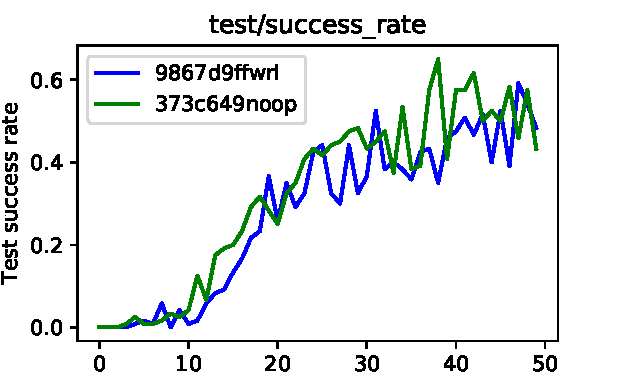
\includegraphics[width=\frac\columnwidth]{media/res/373c649_FetchSlide-v1-noop/test/success_rate.pdf}%
    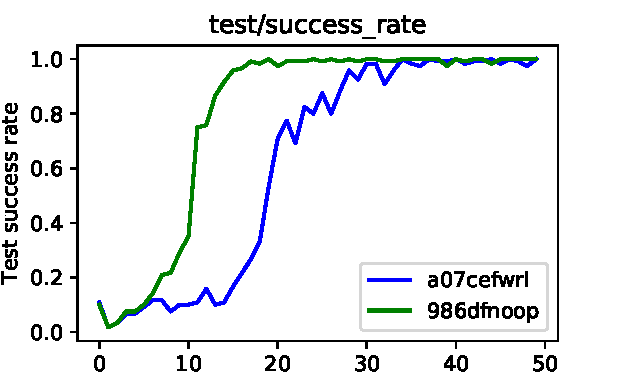
\includegraphics[width=\frac\columnwidth]{media/res/a077c9e_FetchPush-v1-fwrl/test/success_rate.pdf}%
    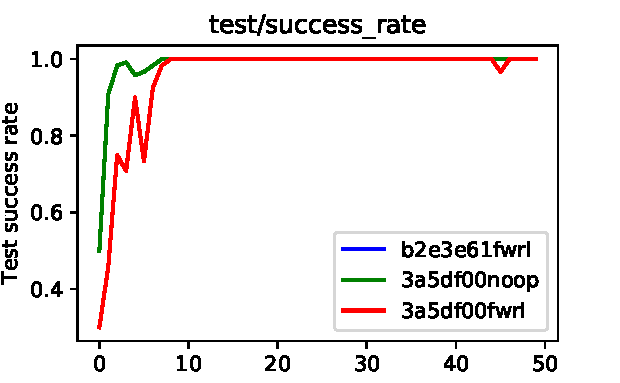
\includegraphics[width=\frac\columnwidth]{media/res/3a5df00_FetchReach-v1-fwrl/test/success_rate.pdf}\\
  \def\frac{0.32}
    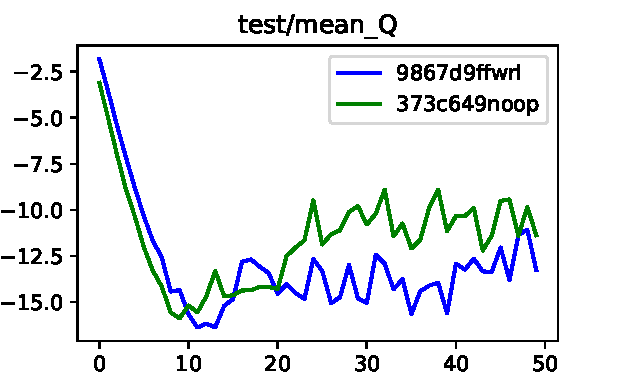
\includegraphics[width=\frac\columnwidth]{media/res/373c649_FetchSlide-v1-noop/test/mean_Q.pdf}%
    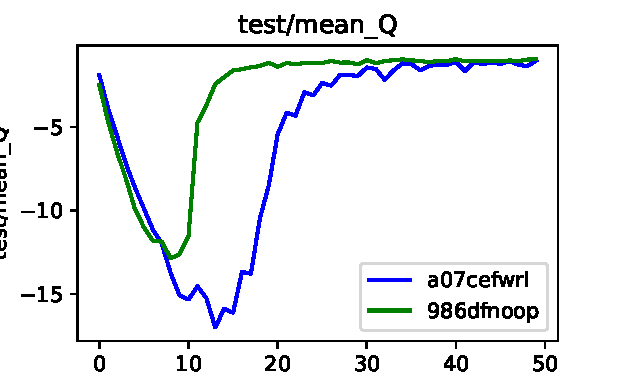
\includegraphics[width=\frac\columnwidth]{media/res/a077c9e_FetchPush-v1-fwrl/test/mean_Q.pdf}%
    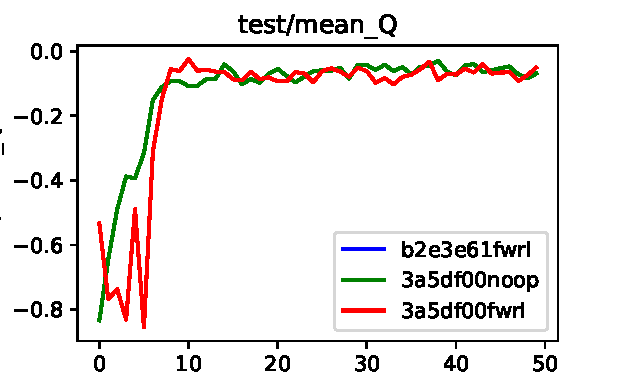
\includegraphics[width=\frac\columnwidth]{media/res/3a5df00_FetchReach-v1-fwrl/test/mean_Q.pdf}
    \caption{Test success rate and Mean Q on Fetch-Slide, Fetch-Push and Fetch-Reach task}
    \label{fig:fetch-slide-success}
\end{figure}


%
\begin{figure}%
  \def\frac{0.24}
  \includegraphics[width=\frac\columnwidth]{media/res/3a90344-FetchReach-v1-stepfwrl-future/test/success_rate.pdf}%
  \includegraphics[width=\frac\columnwidth]{media/res/3a90344-FetchReach-v1-stepfwrl-future/test/mean_Q.pdf}%
  \includegraphics[width=\frac\columnwidth]{media/res/3a90344-FetchReach-v1-stepfwrl-future/train/critic_loss.pdf}%
  \includegraphics[width=\frac\columnwidth]{media/res/3a90344-FetchReach-v1-stepfwrl-future/train/critic_addnl_loss.pdf}\\
  \includegraphics[width=\frac\columnwidth]{media/res/d047a03-FetchReach-v1-stepfwrl-none/test/success_rate.pdf}%
  \includegraphics[width=\frac\columnwidth]{media/res/d047a03-FetchReach-v1-stepfwrl-none/test/mean_Q.pdf}%
  \includegraphics[width=\frac\columnwidth]{media/res/d047a03-FetchReach-v1-stepfwrl-none/train/critic_loss.pdf}%
  \includegraphics[width=\frac\columnwidth]{media/res/d047a03-FetchReach-v1-stepfwrl-none/train/critic_addnl_loss.pdf}
  \caption{
    Algorithms: HER (d047a03noop-future), FWRL (d047a03fwrl-future), StepFWRL
    (3a90344stepfwrl-future). 
    From left: (1): HER helps, Step loss helps,
    (2): FWRL causes over over-optimistic estimates of Q-function
    (3-4): FWRL loss is the major part of critic loss}%
  \label{fig:fwrl-stepfwrl-noop-test-sucess-rate}%
\end{figure}%
% 

%
\begin{figure}%
  \def\frac{0.24}
  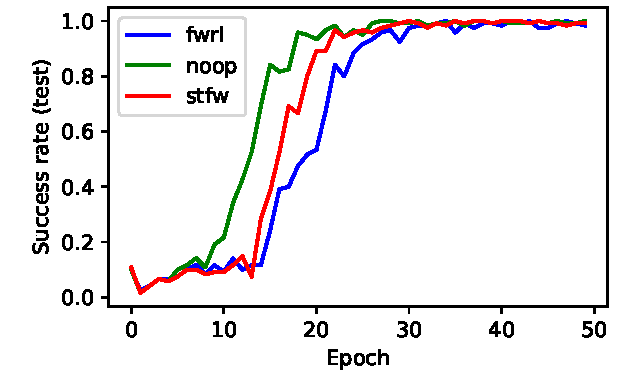
\includegraphics[width=\frac\columnwidth]{media/res/ea0e35b-FetchPush-v1-stfw-future/test/success_rate.pdf}%
  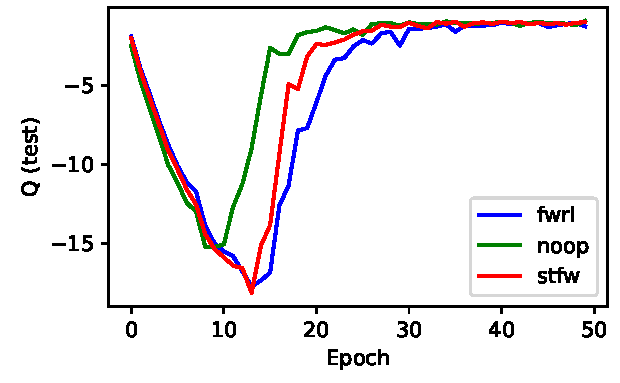
\includegraphics[width=\frac\columnwidth]{media/res/ea0e35b-FetchPush-v1-stfw-future/test/mean_Q.pdf}%
  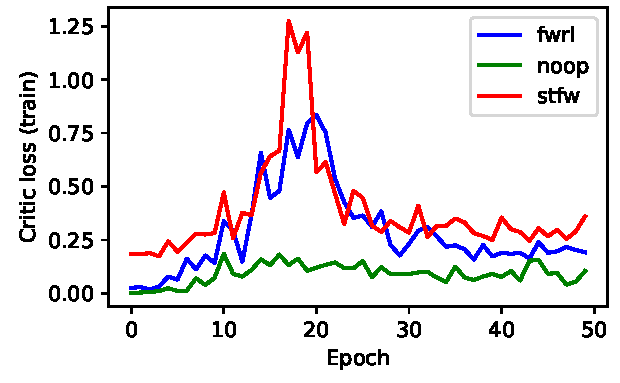
\includegraphics[width=\frac\columnwidth]{media/res/ea0e35b-FetchPush-v1-stfw-future/train/critic_loss.pdf}%
  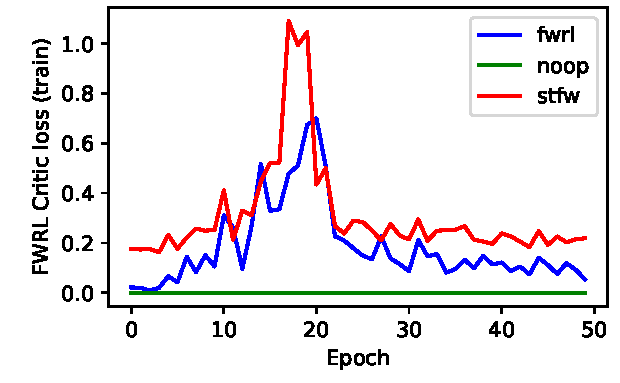
\includegraphics[width=\frac\columnwidth]{media/res/ea0e35b-FetchPush-v1-stfw-future/train/critic_addnl_loss.pdf}\\
  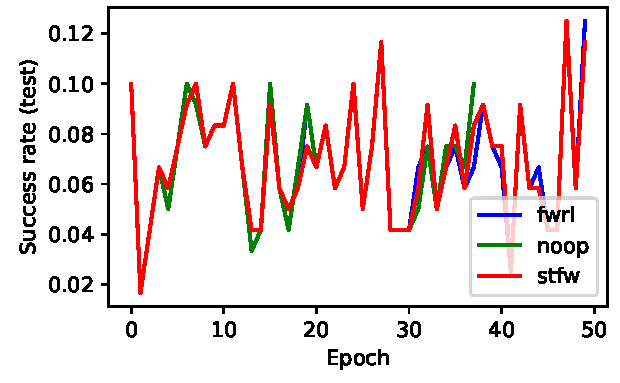
\includegraphics[width=\frac\columnwidth]{media/res/ea0e35b-FetchPush-v1-stfw-none/test/success_rate.pdf}%
  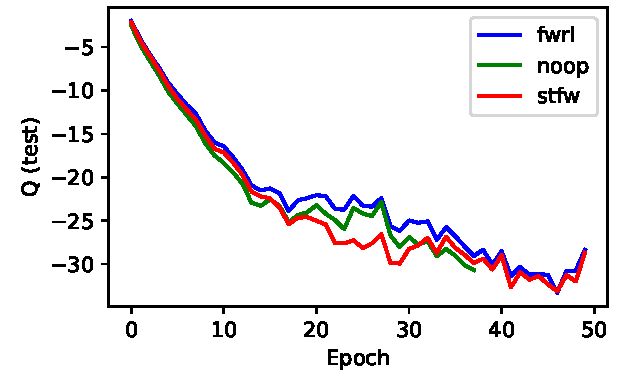
\includegraphics[width=\frac\columnwidth]{media/res/ea0e35b-FetchPush-v1-stfw-none/test/mean_Q.pdf}%
  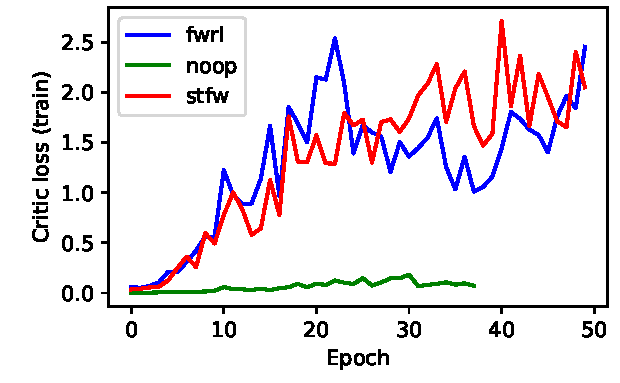
\includegraphics[width=\frac\columnwidth]{media/res/ea0e35b-FetchPush-v1-stfw-none/train/critic_loss.pdf}%
  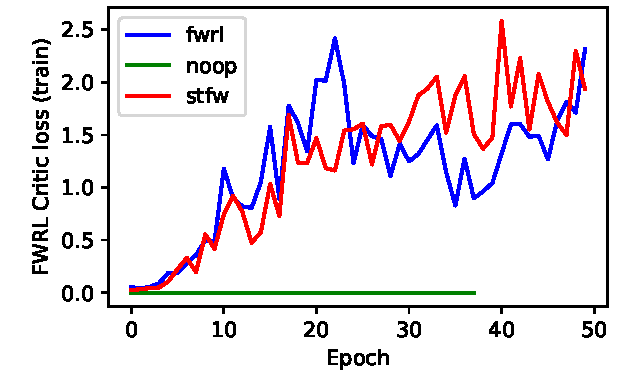
\includegraphics[width=\frac\columnwidth]{media/res/ea0e35b-FetchPush-v1-stfw-none/train/critic_addnl_loss.pdf}
  \caption{
    Algorithms: HER (d047a03noop-future), FWRL (d047a03fwrl-future), StepFWRL
    (3a90344stepfwrl-future). 
    From left: (1): HER helps, Step loss helps,
    (2): FWRL causes over over-optimistic estimates of Q-function
    (3-4): FWRL loss is the major part of critic loss}%
  \label{fig:fwrl-stepfwrl-noop-test-sucess-rate}%
\end{figure}%
% 

\subsection{Over-optimistic estimates of Q-function}
The first attempt to bound the Q-function is to implement the following loss
function,
%
\begin{align}
    \Loss_\fw(\dots) = |
      \fwargs{\state_{s}}{\act_b}{\state_b}{t}{}
      + \fwargs{\state_{bg}}{\policy(\state_s, \state_{bg};\param_\policy)}{\state_s}{t}{}
      - \fwargs{\state_{bg}}{\act_b}{\state_b}{m}{}
      |_+^2.
\end{align}%
% 
However, this cause the algorithm to make over optimistic estimates of expected
reward function. Hence, we add another loss term for upper bound of the Q-function.
%
\begin{align}
    \Loss_\fw(\dots) = |
      \fwargs{\state_{s}}{\act_b}{\state_b}{m}{}
      + \fwargs{\state_{bg}}{\policy(\state_s, \state_{bg};\param_\policy)}{\state_s}{m}{}
      - \fwargs{\state_{bg}}{\act_b}{\state_b}{t}{}
      |_+^2.
\end{align}%
% 

\subsection{Metrics}
The metrics used to quantify and compare agent performance across
FWRL to baseline methods are described here.

\subsubsection{Reward}
As in typical in reinforcement learning, the reward earned per episode by the
agent is treated as a metric of success.

    %\item \textbf{\Loo}\\
    %    We use the metric \Loo as defined in \cite{MiPaViICLR2017} as the ratio
    %    of the time taken to hit the goal for the first time to the average
    %    amount of time taken to hit goals subsequently. It
    %    is the ratio of the exploration time over the exploitation time:
	%	\begin{align}
	%		\text{\Loo} &= 
	%		\frac{(N-1) \tau_1}{\tau_{N} - \tau_1} & \text{if }  N >= 2,
	%	\end{align}%
    %    where $\tau_1, \tau_2, \dots, \tau_N$ are the $N$ time steps at which
    %    the agent reaches the goal.


\subsubsection{Distance-Inefficiency} The distance-inefficiency~\citep{dhiman2018critical} is the ratio of the
      distances travelled by the agent during an episode to the sum of the shortest
      path to the goal at every point of initialization. Mathematically it is defined
      as:
		\begin{align}
			\text{Dist-ineff.} &=
			\frac{ \sum_{i=1}^{N-1} \sum_{k=\tau_i + 1}^{\tau_{i+1} - 1} \|\pos_{k+1} - \pos_{j}\| }
			{ \sum_{i=1}^{N-1} \delta(\pos_{\tau_i + 1}, \pos_g) } ,
		\end{align}%
		%
		where $\delta(\pos_{\tau_i +1}, x_g)$ denotes the shortest path
		distance between spawn location $\pos_{\tau_i+1}$ and goal location
        $\pos_g$. The numerator is the total distance covered by the agent while
        skipping the jumps where the agent gets re-spawned after reaching the
        goal location. The denominator is the total shortest distance during the
        episodes.

\subsection{Baselines}
We compare our FWRL against three baselines: two versions of
Q-Learning~\cite{watkins1992qlearning} and Model based RL (MBRL).

\subsubsection{Q-Learning: QL and QLCAT}
We implement two versions of Q-learning. In the first version, called QL, we
reset the Q-function after every episode. This version of Q-Learning does not
use the prior knowledge of the goal state, but depends upon the goal reward to
build a new Q-function in every episode. In the second version, called QLCAT,
we concatenate the state with the goal location and retain the learned Q-function
function across episodes. 

\subsection{Model-based RL}
We implement a simple version of tabular model-based RL where we maintain a
transition count data-structure $T(\state' | \state, \act)$.
This allows to compute a frequentist estimate of dynamics model.
We also keep a tabular record of the reward from each state-action pair
$R(\state, \act)$. The dynamics model is then used to find the
maximum-reward-path to the goal state.


%
\begin{figure}[h!]%
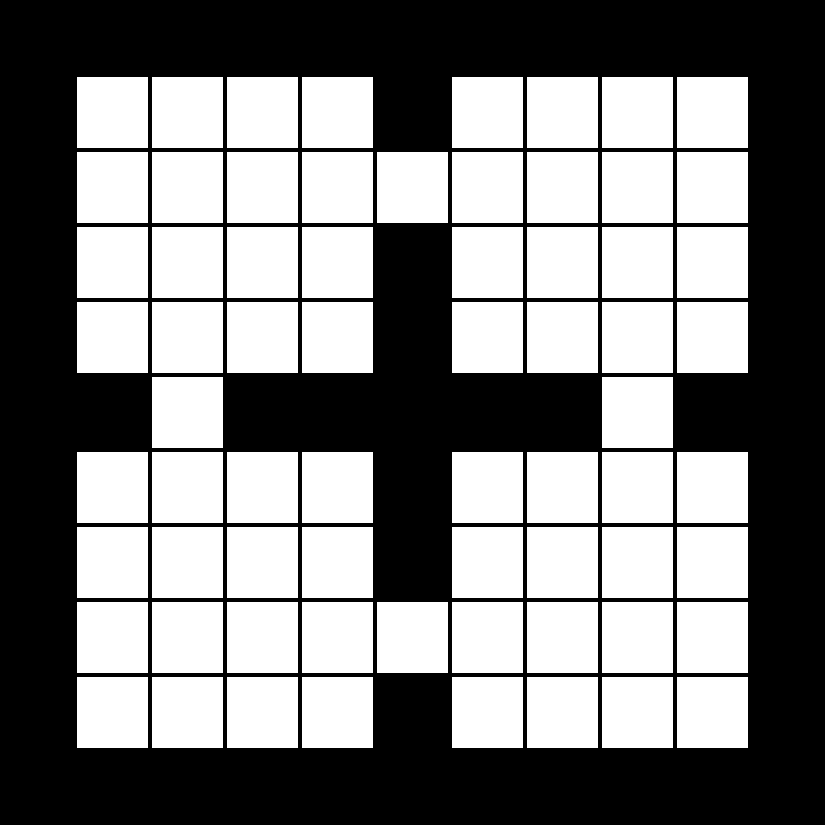
\includegraphics[width=0.48\columnwidth]{media/4-room-grid-world.pdf}
\hfill
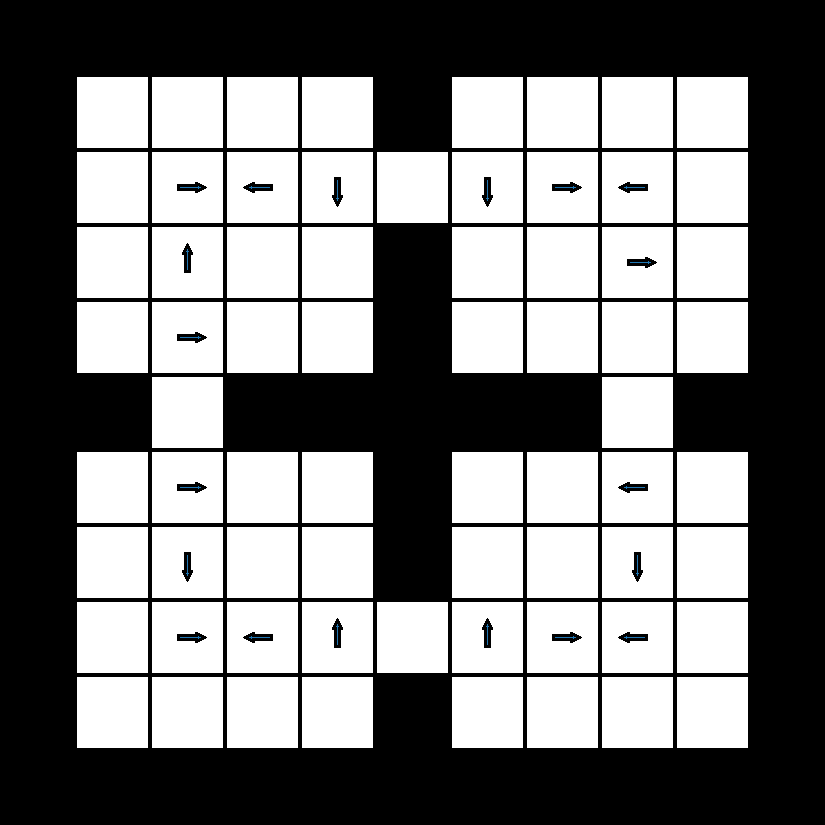
\includegraphics[width=0.48\columnwidth]{media/4-room-windy-world.pdf}%
\caption{Left: Four room grid world. Right: Four room windy grid world with wind direction shown by arrows. The windy pushes the agent in the direction of wind with 0.25 probability irrespective of the action taken.}
\label{fig:four-room-grid-world}%
\end{figure}%
%
